\documentclass[conference]{IEEEtran}
\usepackage[utf8]{inputenc}
\usepackage{amsmath}
\usepackage{changepage}
\usepackage{graphicx}
\usepackage{float}
\usepackage{amssymb}

\title{Open Source Software Framework for Indoor Geolocation Using 802.11 Protocol}
\author{Authors Name }
\date{April 2018}

\begin{document}

\maketitle
\begin{abstract}
Indoor Geolocation Positioning is an emerging new technology that ha and edge over others due to its ability the exact location of a person.of 1 in 4 Americans over the age of 65 fall every year. [1] Most of these falls
are very serious and can result in major mobility injuries and/or death. The
shorter the amount of time it takes for fall victims to get medical attention, the
higher their odds of recovery are. As such, it would be very beneficial to develop a
device capable of identifying the location of a victim within a building or indoor
environment using existing infrastructure. 
\newline This paper designs and implements a open Source platform to derive the exact location of a person using 802.11 protocol.
\end{abstract}
\section{Introduction}
\newline According to the Centers for Medicare and Medicaid Services, healthcare in the United States has seen a tremendous growth in past decade. It projects 5.9\% growth increase in 2018 and projects to see 19.9\% National Health spending as a share of GDP. The maximum percentage of this is needed by people above the age of 55 which comprise approximately 29\% of the population in America [1]. The primary reason for injuries in elderly people are the falls due to their debility with respect to their age. Some of this injuries can be fatal or may create a psyche of fear in the individual resulting in them losing the ability to walk properly after the fall. Many Algorithms and Embedded Technologies have been in research and development for the past several years which aim to work towards the basic goal of detecting a fall and reporting the location of the fallen individual to the respective authority.
\newline Many IoT devices that have previously been developed require the employment of GPS(R)[REFERENCE] to locate the individual. However, the indoor error of GPS is approximately XXXX [REFERENCE], which far exceeds the the threshold for room-level location derivation. In addition, GPS does not derive an altitude for the user's location which prevents floor-level determination from taking place. Other implementations make use of proprietary hardware/software solutions which cost large sums of money to deploy and maintain.[REFERENCE]
\newline This paper sketches the development of an Open Source Software Platform capable of tracking the movements of individuals using existing 802.11 WiFi(R) Infrastructure. The modularity of the Software Framework developed, and it's strong use of C++11 Design Principles, also enables it to be easily adapted to a variety of hardware platforms and radio technologies such as Bluetooth(R)[INSERT REFERENCE] or LoraWAN[INSERT REFERENCE].
\begin{figure}[H]
    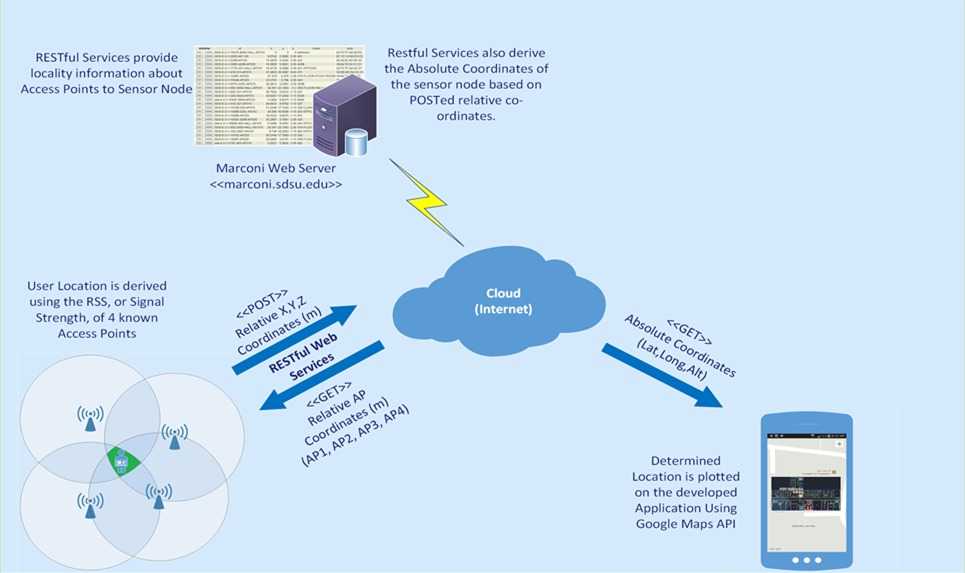
\includegraphics[width=9 cm,height=5.5 cm]{2018-05-10-PHOTO-00000077.jpg}
    \caption{Overview}
    \end{figure}
    \ListofFigures
\section{Architecture}
The main framework architecture of this project has four components viz Node Reader Module, Node Scanner Module, Location Derivation Module and the Rest Module. Each of the module were developed separately
\begin{figure}[H]
    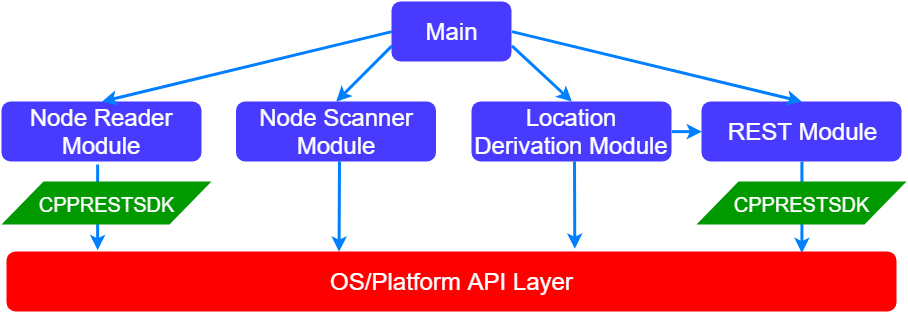
\includegraphics[width=9 cm,height=5.5 cm]{Pink_Panther_Architecture.png}
    \caption{Architecture}
    \end{figure}
    \ListofFigures
    
\section{Indoor Tracking}
\noindentThe ability to identify the geographic location of an individual residing outside of a building by latitude, longitude, and altitude is easily accomplished using a relatively inexpensive GPS receiver. Typical commercially available receivers for under \$100 can provide coordinates within a sampling time of the 30s to an accuracy of ±3m. For example, the Copernicus II 12-channel GPS module from Trimble is under \$70 and can provide updated coordinates with a period of 3s. GPS receivers typically use a carrier wave in the L1 band at 1575.42 MHz on which navigation messages are modulated. Unfortunately, such microwave signals are significantly attenuated by building roofs and walls, rendering GPS unusable indoors. [2]
The measurement of  the position of an individual indoors can be accomplished using different mechanisms such as radio signals, magnetic fields, and sound waves. Newer, emerging technologies employ computer vision to identify objects in the field of a camera's view. The vision system can then measure distances in between recognized objects, and between the user and recognized objects. These measurements provide a system with depth perception and can identify how far a user is away from a surface or other rigid body in a field of view.
This research project utilizes radio signals, specifically radio signals from 802.11 Wi-fi Access Points. After calculating the known location of these Access Points and the signal strength at the receiver,the distance can be derived using a modification of the free space equation. Here we are using four access point to dervive the location of user by caluculating the distance between them using the trilateration technology.
\subsubsection{Trilateration}
Trilateration technique is used to determine the relative location of a particular user in an offline fashion with the help of location of Access points. Indoor  positioning  will  be  accomplished  by  measuring  the  Received  Signal  Strength  (͞RSS͟)  of  the  device,  reported  by  the  WiLink  8  module,  from  several  different  Wi-Fi  access  points  (͞APs͟)  within  32m  of  the  user.    Typically,  the  received  signal  power  within  one  meter  of  an  AP  will  be  approximately  -30  dBm,  and  close  to  -90  dBm  at  a  distance  of  32m. The RSS can be  modeled using  equation  (1)  
\begin{equation}
RSS = 10N*\log_{10}D-A  
\end{equation}
where: 
\begin{conditions}
N & = Signal propagation constant\\
A & = received Signal power at 1 meter\\
D & = distance in meters\\
\end{conditions}
\newline With  four  APs,  one  can  use  trilateration  to  locate  a  user  using  four  distances  computed  from  four  RSS  values.    Let  ( x , y , z )  represent  the  unknown  location  of  a  user  and $(d_1,  d_2,  d_3,  d_4)$represents four distance values obtained from the measured RSS between user's WIPS and Four APs. The System of Euclidian  distances  between  the  user  and  four  APs  is  given  by  equations below
\begin{equation}
x-x_1^2 + y-y_1^2 + z-z_1^2 =d_1^2
\end{equation}
\begin{equation}
 x-x_2^2 + y-y_2^2 + z-z_2^2 =d_2^2 
\end{equation}
\begin{equation}
 x-x_3^2 + y-y_3^2 + z-z_3^2 =d_3^2 
\end{equation}
\begin{equation}
 x-x_4^2 + y-y_4^2 + z-z_4^2=d_4^2 
 \end{equation}
 \newline Subtracting each rows 2,3,4 each from row 1,we have\\
$2(x_2 - x_1) + 2(y_2 - y_1)y + 2 (z_2 - z_1)z = x_2^2 - x_1^2 + y_2^2 - y_1^2 + z_2^2 - z_1^2 - d_2^2 +d_1^2 $\\
\\
$2(x_3 - x_1) + 2(y_3 - y_1)y + 2 (z_3 - z_1)z = x_3^2 - x_1^2 + y_3^2 - y_1^2 + z_3^2 - z_1^2 - d_3^2 +d_1^2$\\
\\
$2(x_4 - x_1) + 2(y_4 - y_1)y + 2 (z_4 - z_1)z = x_4^2 - x_1^2 + y_4^2 - y_4^2 + z_4^2 - z_1^2 - d_4^2 +d_1^2$\\\\
The System can be expressed in Ax=b matrix form as
\[ \left[ \begin{array}{ccc}
(x_2 - x_1) & (y_2 - y_1) & (z_2 - z_1) \\
(x_3 - x_1) & (y_3 - y_1) & (z_3 - z_1) \\
(x_4 - x_1) & (y_4 - y_1) & (z_4 - z_1) \\
\end{array} \right] 
%
\left[ \begin{array}{c}
x \\
y\\
z\\
\end{array} \right] 
% 

\left\[= 1/2\]
\left[ \begin{array}{c}

x_2^2 - x_1^2 + y_2^2 - y_1^2 + z_2^2 - z_1^2 - d_2^2 + d_1^2 \\
x_3^2 - x_1^2 + y_3^2 - y_1^2 + z_3^2 - z_1^2 - d_3^2 + d_1^2 \\
x_4^2 - x_1^2 + y_4^2 - y_1^2 + z_4^2 - z_1^2 - d_4^2 + d_1^2 \\
\end{array} \right]
\]
\newline and  solved  using  a  Gauss- Newton least  squares  approximation. 
\begin{equation}
(A^TA)X = A^Tb
\end{equation}
Multipath  effects,  co-channel  interference  (͞CCI͟),  and  adjacent-channel  interference  (͞ACI͟)  can  reduce  the  SNR,  resulting  in  location  measurement  error.    We  will  investigate  approaches  to  mitigate  location  measurement  error  using  repeated  sampling,  averaging,  and  other  techniques,  once  we  construct  a  prototype  and  conduct  several  experiments  in  a  controlled  laboratory  setting  where  we  can  tune  and  calibrate  the  prototype.Additional  APs  can  be  incorporated  into  the  user's  environment  to  reduce  trilateration  error.        APs  in  excess  of  three  or  more  form  an  over-determined  system  of  equations.    We  can  form  three  equations  in  three  unknowns  by  doing  additional  row  operations,  as  we  have  shown  in  (4).    We  will  evaluate  the  patient's  environment  and  determine  the  optimal  placement  of  three  or  more  APs  to  minimize  trilateration  error.      We  will  also  map  the  patient's  environment  to  a  Cartesian  coordinate  system  so  a  determined  location  ( x , y ,  z) can  be  quickly  located  by  support  staff,  should  an  emergency  arise. 
\subsubsection{Kalman Filter}
RSS (Received Signal Strength) value depends directly, and only, on the distance between the 802.11 Wi-Fi transmitter and the receiver – in an ideal system. In reality, however, Multipath interference, Electromagnetic interference and signal fading all play a significant role in causing fluctuations in the Received Signal Strength. As such, it is required that the RSS values are filtered in the time domain such as to mitigate the effect of such noise. One such method is through the use of a Kalman Filter with Measurement Covariance (R) and Process Covariance (Q) parameters as shown below. 
\begin{equation}
_p = _p + _q;
\end{equation}
\begin{equation}
 _k = _p / (_p + _r);
\end{equation}
\begin{equation}
_x = _x + _k * (measurement - _x);
\end{equation}
\begin{equation}
 _p = (1 - _k) * _p;
\end{equation}
where:
\begin{conditions}
double\_q & is Process noise covariance \\
double\_q\_init; double\_r & is Measurement noise covariance\\
double\_r\_init;double\_x & value\\
double\_p & estimation error covariance
double\_p\_init ;double\_k & Kalman gain\\
\end{conditions}
\newline Measurement Covariance is the standard deviation of a set of measured results – determined to be 2.36 - and Process Covariance is the susceptibility of the system to change - determined to be 0.0001. The implemented Kalman Filter is a function of these parameters, the current RSS and the RSS history. 
\subsection{Middle Ware}
\subsubsection{RESTful Web Services}
Represenatational State transfer style web service was build on the existing frame work to access the data.
\subsection{Back end Database}


\section{Mobile App}
The mobile application, developed using Android Studio, displays a visual representation of the sensor’s real-world location. The app employs the Google Maps 2.0 API extensively to achieve this, with an overlay of the architectural plans for target buildings. A consume web services function was defined which requests a string response from the implemented RESTful web services on Marconi. A function was defined named process JSON which breaks down the JSON string into variables that can be manipulated, such as timestamp, alt, latitude, and longitude. Altitude was not used, however for the latitude and longitude other function named modification was created with parameters of the string timestamp, string data, double latitude, and double longitude. A function, modification, was defined which modifies the last known location of the user (blue dot) by setting the latitude and longitude based on the calculated data provided by the RESTful API. The camera (the focus of the screen in the app) is also moved according to the new data within this function to focus on the user (blue dot).
\begin{figure}[H]
    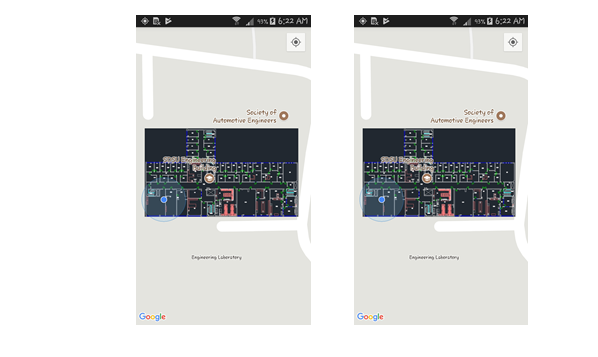
\includegraphics[width=8cm,height=5cm]{2018-05-10-PHOTO-00000078.png}
    \caption{Working App}
    \end{figure}
    \ListofFigures
\section{Results}
Kalman Filter results
according to the new data within this function to focus on the user (blue dot).
\begin{figure}[H]
    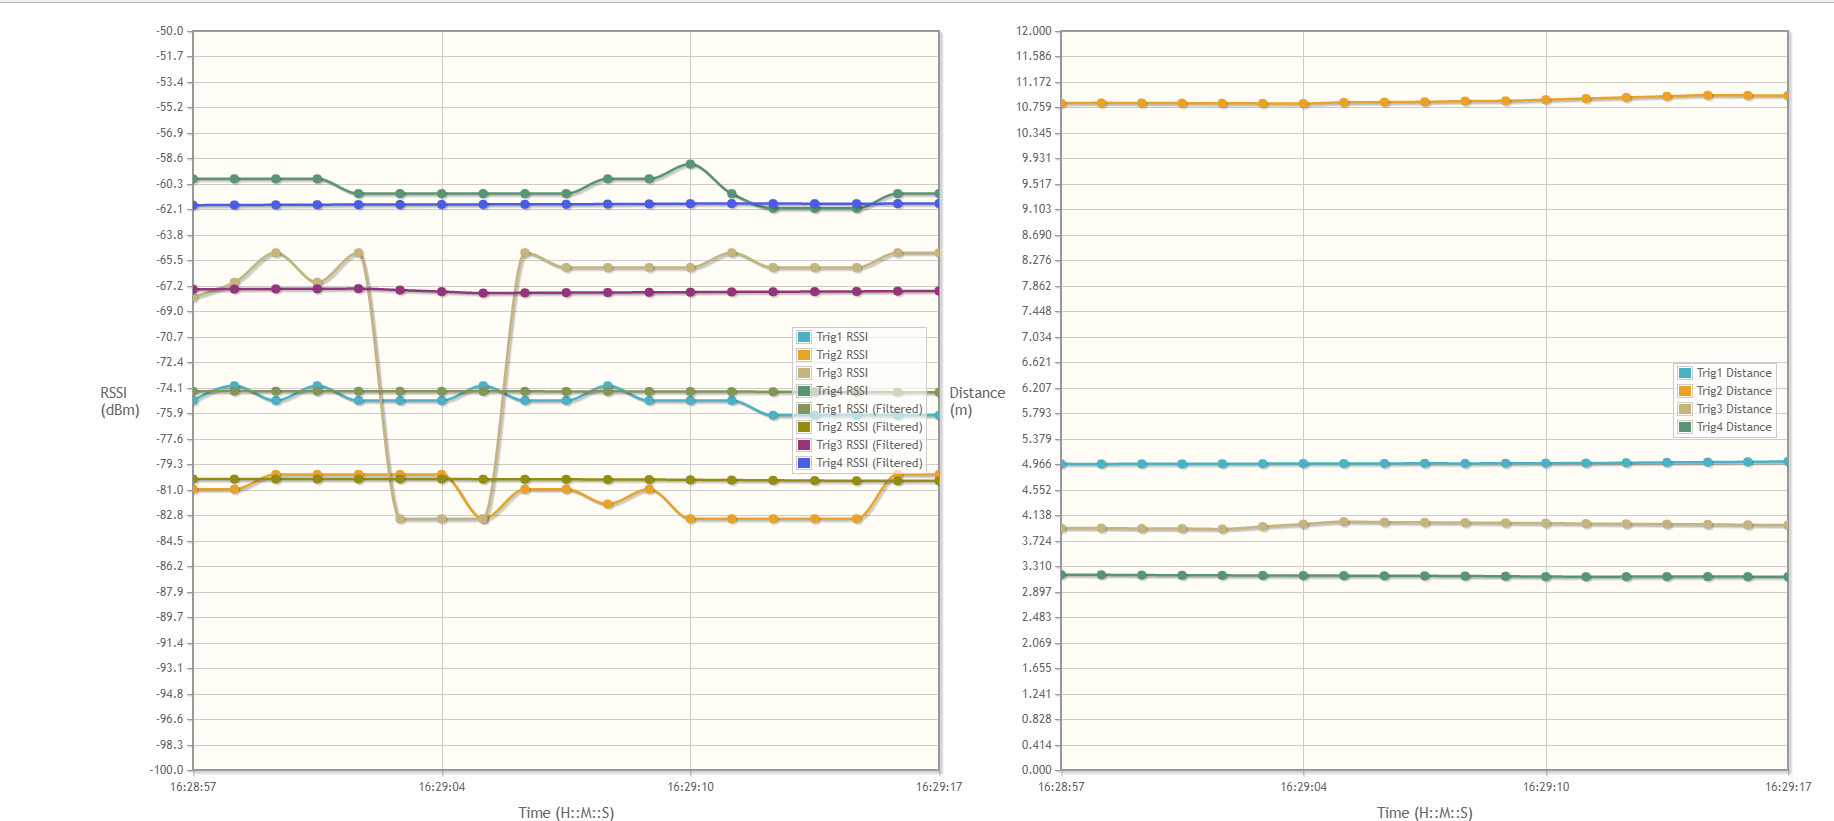
\includegraphics[width=8cm,height=5cm]{2018-05-10-PHOTO-00000079.png}
    \caption{Kalman Results}
    \end{figure}
    \ListofFigures
\section{Conclusion}

\section{References}
[1] http://money.cnn.com/2018/01/30/news/economy/health-care-costs-eating-the-economy/index.html
\end{document}
